\chapter{評価}
\label{evaluation}

本章では第\ref{implementation}章ので記述した3つの実験の結果を述べ考察を行う。

\section{実験1の結果 既存の活性化関数との比較実験}
\label{evo1}
本節では\ref{exp1}節で示した設定もとに実験を行い、その結果を述べ各データセットにおいてどの程度の学習性能を示したか結論を述べる。

\subsection{irisでの比較実験}
\label{ev:iris}

第4章の\ref{impl:iris}項で設定した実験を行い、結果を以下にまとめた。
\subsubsection{設定1及び設定2の結果}

irisを用いた活性化関数の比較結果を表\ref{result:iristable}に記す。

\begin{table}[htbp]
    \begin{center}
        \caption{irisの設定1及び設定2のAccuracy}
        \label{result:iristable}
        \vspace{2mm} 
        \begin{tabular}{|c|c|c|}
            \hline
            活性化関数  & 設定1のAccuracy &  設定2のAccuracy \\
            \hline
            K-AF            & 72.0 & 26.0 \\
            \hline
            Sigmoid            & 68.0 & 77.3\\
            \hline
            Tanh            & 20.0 & 53.0\\
            \hline
            ReLU        &  49.6 &  38.3\\
            \hline
            Swish           & 87.3 & 47.3 \\
            \hline
            Mish           & 60.0 & 65.0 \\
            \hline
    
        \end{tabular}
    \end{center}
\end{table}


\subsubsection{設定1及び設定2のValidationLoss}
\label{iris:loss}


ValidationLossのログデータを図\ref{iris:loss_image1}と図\ref{iris:loss_image2}に示す。

\begin{figure}[hbtp]
    \begin{center}
        \begin{tabular}{c}
            \begin{minipage}{0.5\hsize}
                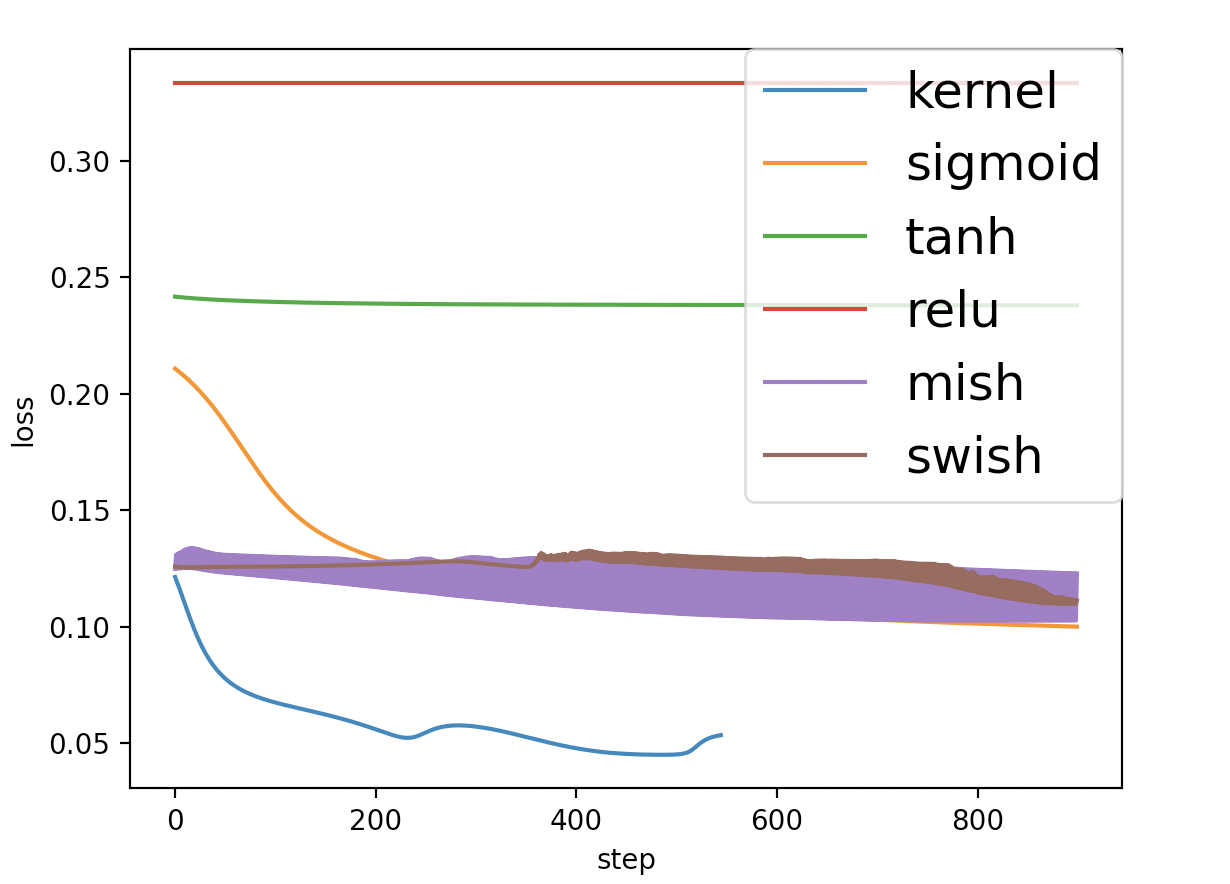
\includegraphics[clip, width=7cm]{asset/iris_0.1_1000_3_02_sgd_non_kaiming_uniform.png}
                    \caption{irisの設定1の結果のValidationLoss}
                    \label{iris:loss_image1}
            \end{minipage}
            \hspace{10pt}
            \begin{minipage}{0.5\hsize}
                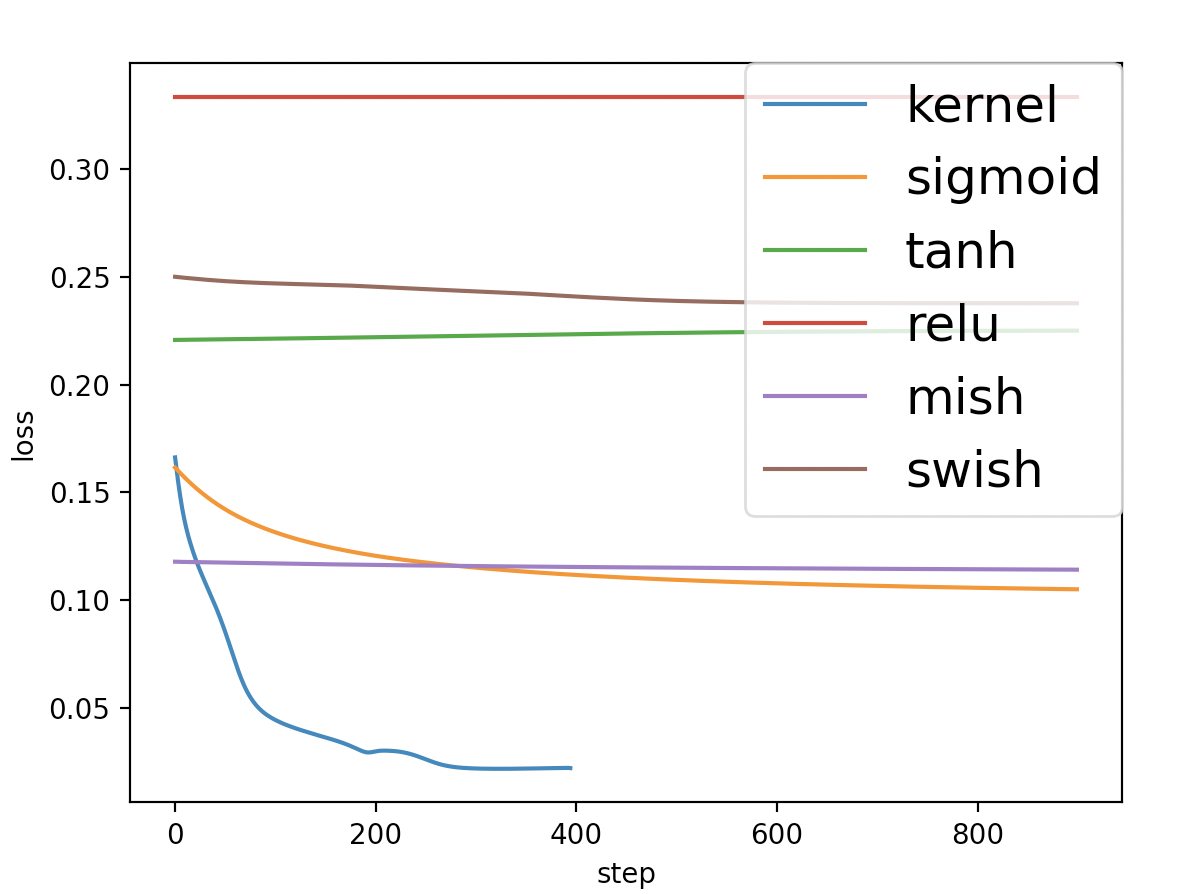
\includegraphics[clip, width=7cm]{asset/iris_0.1_1000_3_02_sgd_l2_kaiming_uniform.png}
                    \caption{irisの設定2の結果のValidationLoss}
                    \label{iris:loss_image2}
            \end{minipage}
        \end{tabular}
    \end{center}
\end{figure}


\subsubsection{irisでの実験結果の考察}


irisは最も単純な分類問題の一つであるが結果\ref{result:iristable}を分析すると特に学習を効率的にするテクニックを使わない場合は良い精度が出せている。
Swishが高い性能を出していることも確認できる。
また、L2のRegularizerを入れるとかなり精度が下がってしまうことから、K-AFは既存の学習テクニックとの組み合わせでは精度が向上しないことが確認できる。






\subsection{digitsでの比較実験}
\label{ev:digitsでの比較実験}
第4章の\ref{impl:digits}項で設定した実験を行い、結果を以下にまとめた。
\subsubsection{設定1及び設定2の結果}
\label{digits:result}

digitsを用いた活性化関数の比較結果を表\ref{result:digitstable}に記す。

\begin{table}[htbp]
    \begin{center}
        \caption{digitsの設定1及び設定2のAccuracy}
        \label{result:digitstable}
        \vspace{2mm} 
        \begin{tabular}{|c|c|c|}
            \hline
            活性化関数              & 設定1のAccuracy &  設定2のAccuracy \\
            \hline
            K-AF            & 91.6 & 60.0 \\
            \hline
            Sigmoid            & 92.0 & 68.6\\
            \hline
            Tanh            & 95.6 & 89.6 \\
            \hline
            ReLU        & 38.0 & 54.3 \\
            \hline
            Swish           & 50.3 & 56.6 \\
            \hline
            Mish           & 55.6 & 53.3 \\
            \hline
    
        \end{tabular}
    \end{center}
\end{table}


\subsubsection{設定1及び設定2のValidationLoss}
\label{digits:loss}

ValidationLossのログデータを図\ref{digits:loss_image1}と図\ref{digits:loss_image2}に示す。


\begin{figure}[hbtp]
    \begin{center}
        \begin{tabular}{c}
            \begin{minipage}{0.5\hsize}
                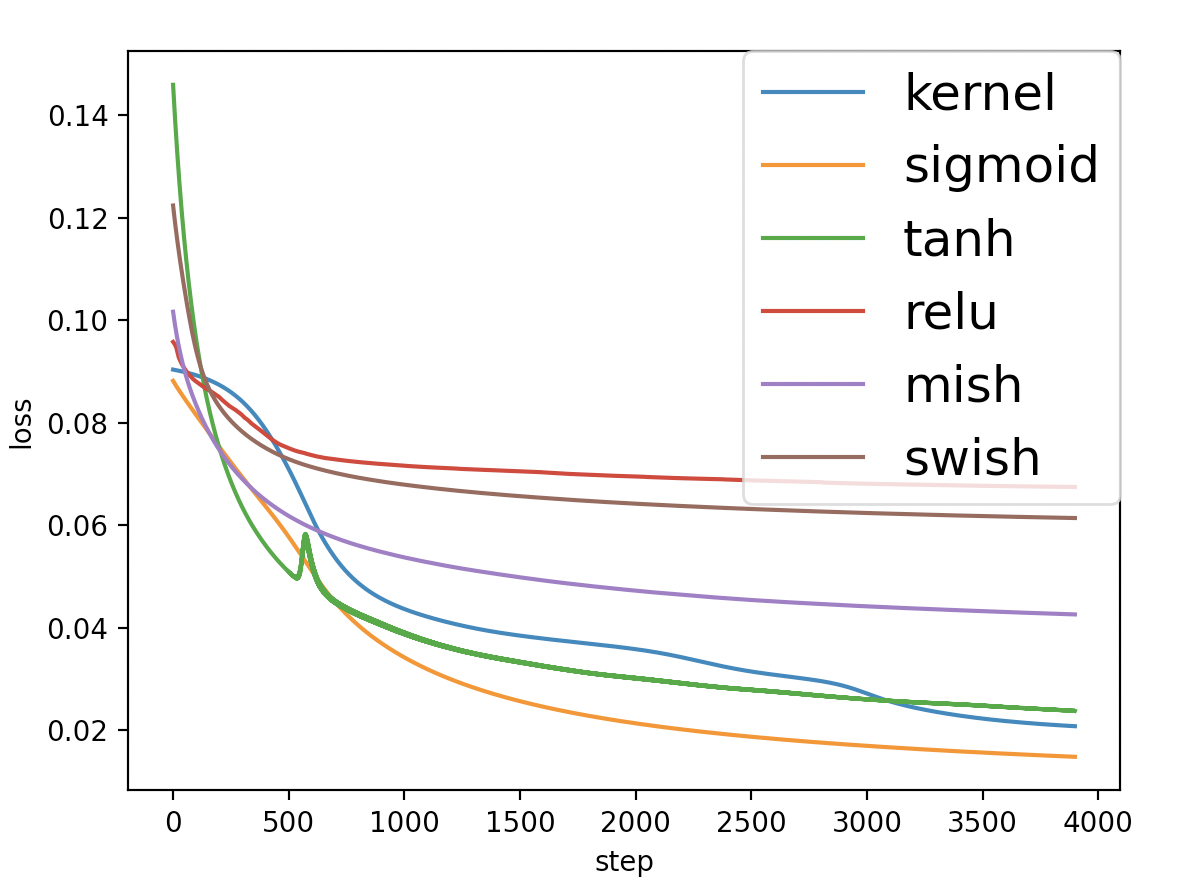
\includegraphics[clip, width=7cm]{asset/digits_0.01_4000_3_002_sgd_non_kaiming_uniform.png}
                    \caption{digitsの設定1の結果のValidationLoss}
                    \label{digits:loss_image1}
            \end{minipage}
            \hspace{10pt}
            \begin{minipage}{0.5\hsize}
                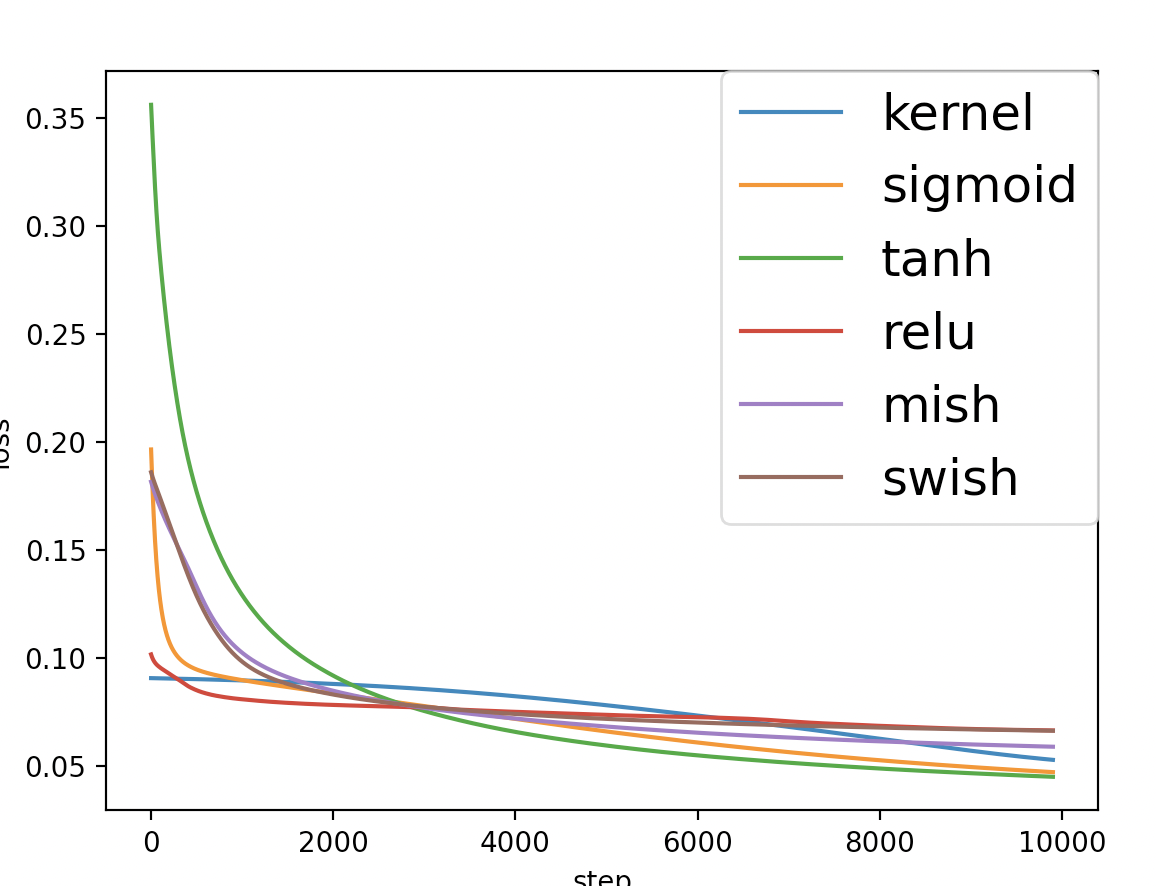
\includegraphics[clip, width=7cm]{asset/digits_0.001_10000_3_002_adam_non_kaiming_uniform.png}
                    \caption{digitsの設定2の結果のValidationLoss}
                    \label{digits:loss_image2}
            \end{minipage}
        \end{tabular}
    \end{center}
\end{figure}


\subsubsection{digitsでの実験結果の考察}
結果\ref{digits:result}を確認すると設定1の場合では91.6\%とSigmoidやTanhといったラベリングによく用いられる活性化関数に匹敵する精度を出せた。ReLU、Mish、Swish等のの上限値が存在しない関数よりも遥かに良い性能を出すことができた。
設定2の場合でもSigmoidやTanhほどの成果は出なかったものの、上限値が存在しない関数よりはいい性能を出すことができた。

ValidationLossのグラフ\ref{digits:result}を確認すると、設定の1,2共に順調に下に推移してることが確認できる。
設定1の方で途中でTanhを追い抜いている理由は、活性化関数の形が急激に変わる瞬間があるからだと推測できる。


\subsection{wineでの実験と設定}
\label{ev:wineでの実験と設定}

第\ref{implementation}章の\ref{impl:wine}項で設定した実験を行い、結果を以下にまとめた。
\subsubsection{設定1及び設定2の結果}

wineを用いた活性化関数の比較結果を表\ref{result:winetable}に記す。


\begin{table}[htbp]
    \begin{center}
        \caption{wineの設定1及び設定2の結果Accuracy}
        \label{result:winetable}
        \vspace{2mm} 
        \begin{tabular}{|c|c|c|c|}
            \hline
            活性化関数              & 設定1のAccuracy &  設定2のAccuracy \\
            \hline
            K-AF            & 72.0 & 27.0 \\
            \hline
            Sigmoid            & 33.3 & 43.0\\
            \hline
            Tanh            & 33.3 & 38.3\\
            \hline
            ReLU        & 33.3 & 0.0\\
            \hline
            Swish           & 33.3 & 27 \\
            \hline
            Mish           & 33.3 &  27.0\\
            \hline
    
        \end{tabular}
    \end{center}
\end{table}


\subsubsection{設定1及び設定2のValidationLoss}
\label{wine:loss}

ValidationLossのログデータを図\ref{wine:loss_image1}と図\ref{wine:loss_image2}に示す。

\begin{figure}[hbtp]
    \begin{center}
        \begin{tabular}{c}
            \begin{minipage}{0.5\hsize}
                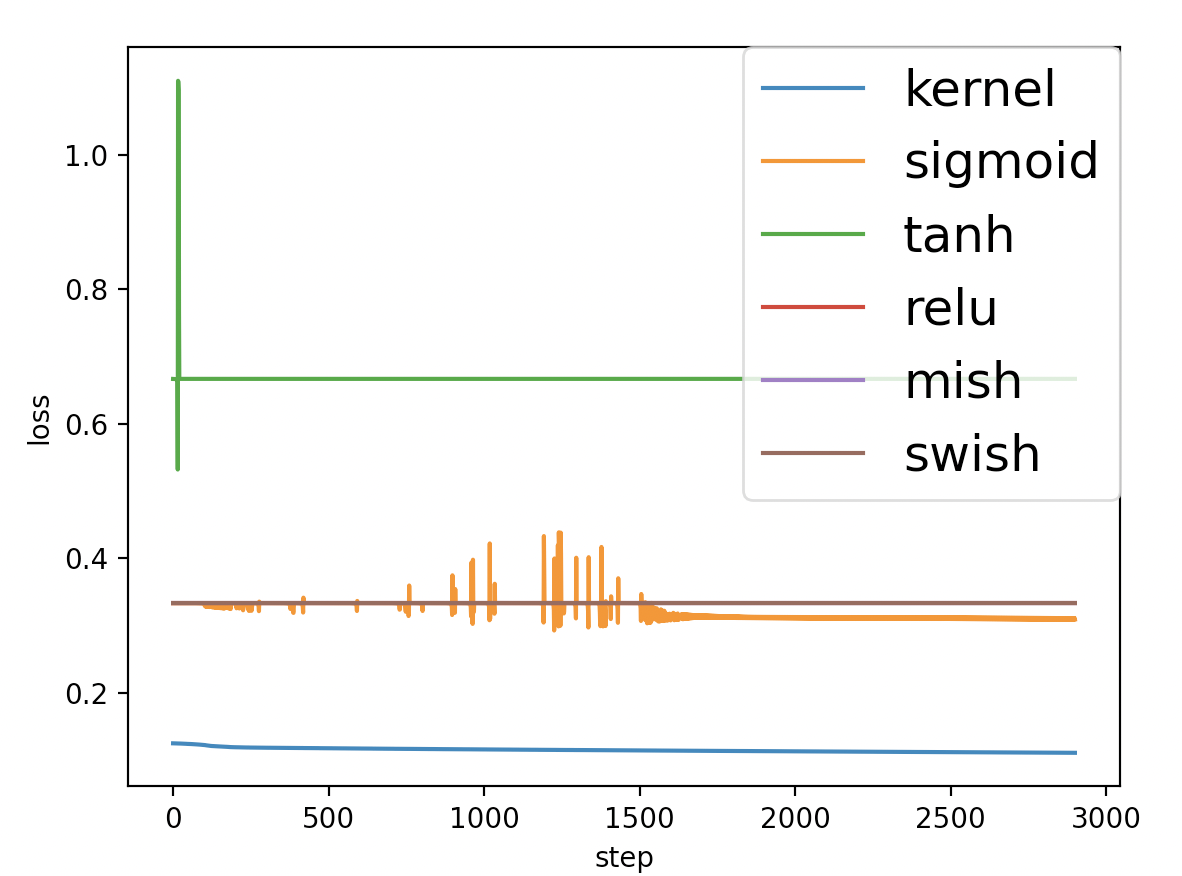
\includegraphics[clip, width=7cm]{asset/wine_0.001_3000_3_015_sgd_non_kaiming_uniform.png}
                    \caption{wineの設定1の結果のValidationLoss}
                     \label{wine:loss_image1}
            \end{minipage}
            \hspace{10pt}
            \begin{minipage}{0.5\hsize}
                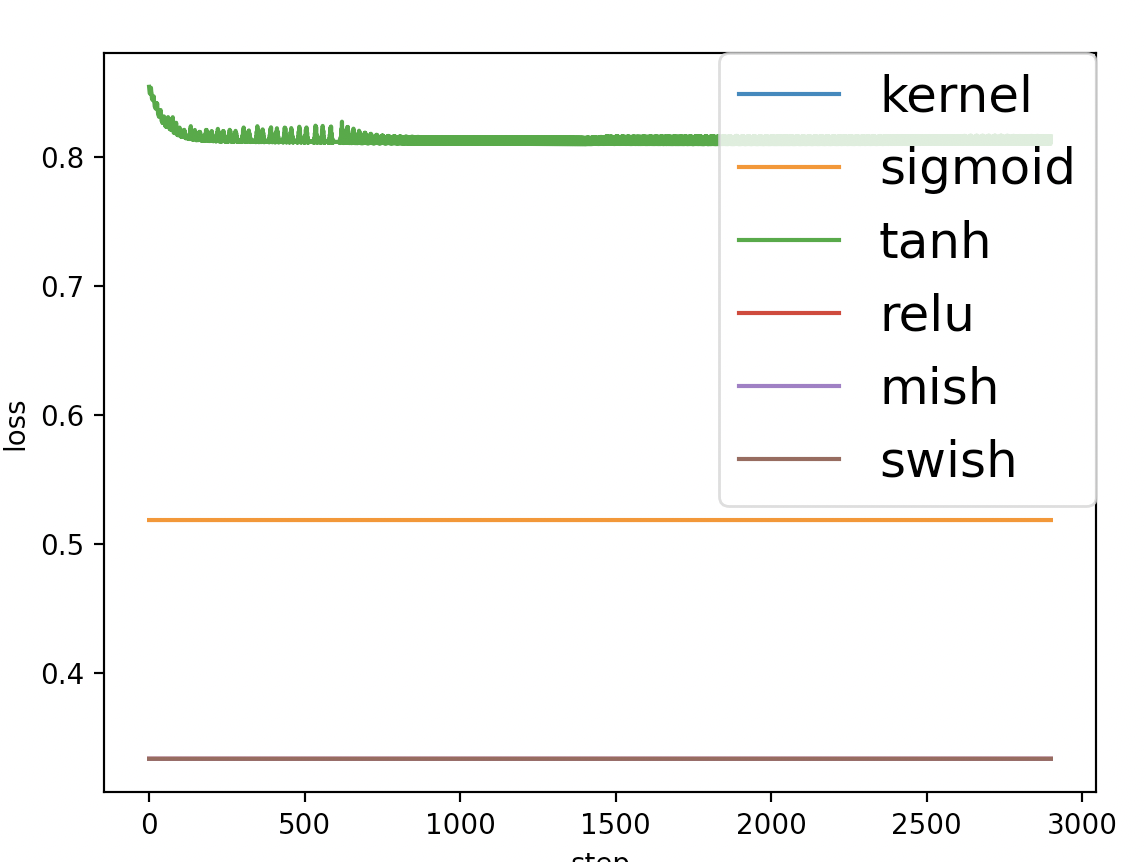
\includegraphics[clip, width=7cm]{asset/wine_0.001_3000_3_015_adam_non_kaiming_uniform}
                    \caption{wineの設定2の結果のValidationLoss}
                     \label{wine:loss_image2}
            \end{minipage}
        \end{tabular}
    \end{center}
\end{figure}


\subsubsection{wineでの実験結果の考察}
結果\ref{result:winetable}を確認するとwineはもともと決定木に使用されるデータセットのためか、設定1ではK-AF以外では勾配爆発してしまっていることが考えられる。
また、設定2はOptimizerをAdamに変えただけ、学習が失敗することが明らかになった。
全体を通してもSGDのK-AFが最大のAccuracyを出している。







\subsection{bostonでの比較実験}
\label{ev:bostonでの比較実験}

第4章の\ref{impl:boston}項で設定した実験を行い、結果を以下にまとめた。
\subsubsection{設定1及び設定2の結果}

bostonを用いた活性化関数の比較結果を表\ref{result:bostontable}に記す。


\begin{table}[htbp]
    \begin{center}
        \caption{bostonの設定1及び設定2のMSE}
        \label{result:bostontable}
        \vspace{2mm} 
        \begin{tabular}{|c|c|c|}
            \hline
            活性化関数              & 設定1のMSE &  設定2のMSE \\
            \hline
            K-AF            & 49.4 & 69.4 \\
            \hline
            Sigmoid            & 523.0 & 541.4 \\
            \hline
            Tanh            & 540.6 &  567.8 \\
            \hline
            ReLU        & 359.2 & 473.4 \\
            \hline
            Swish           & 257.0 & 372.4 \\
            \hline
            Mish           & 360.0 & 472.4 \\
            \hline
    
        \end{tabular}
    \end{center}
\end{table}


\subsubsection{設定1及び設定2のValidationLoss}
\label{boston:loss}

ValidationLossのログデータを図\ref{boston:loss_image1}と図\ref{boston:loss_image2}に示す。

\begin{figure}[hbtp]
    \begin{center}
        \begin{tabular}{c}
            \begin{minipage}{0.5\hsize}
                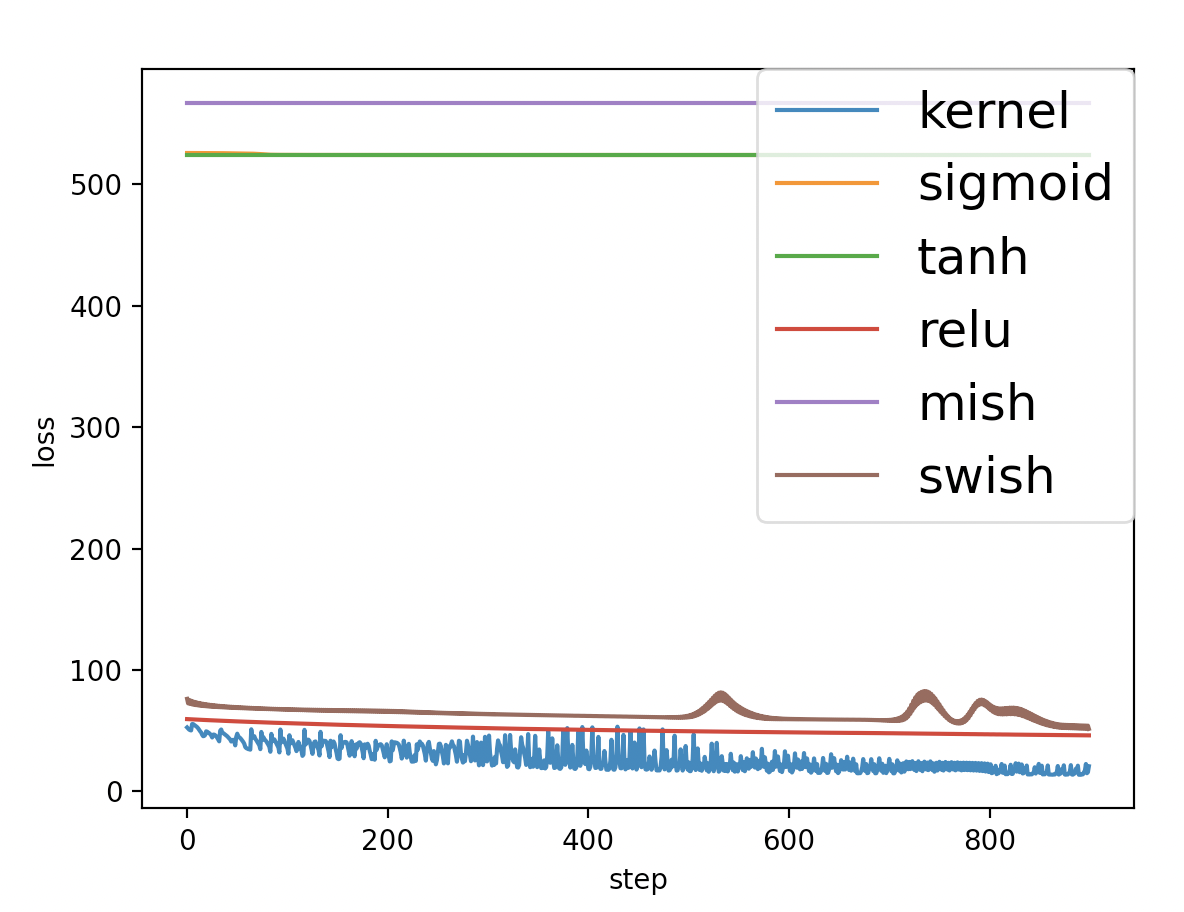
\includegraphics[clip, width=7cm]{asset/boston_0.00001_1000_3_005_sgd_non_kaiming_uniform.png}
                    \caption{bostonの設定1の結果のValidationLoss}
                    \label{boston:loss_image1}
                    
            \end{minipage}
            \hspace{10pt}
            \begin{minipage}{0.5\hsize}
                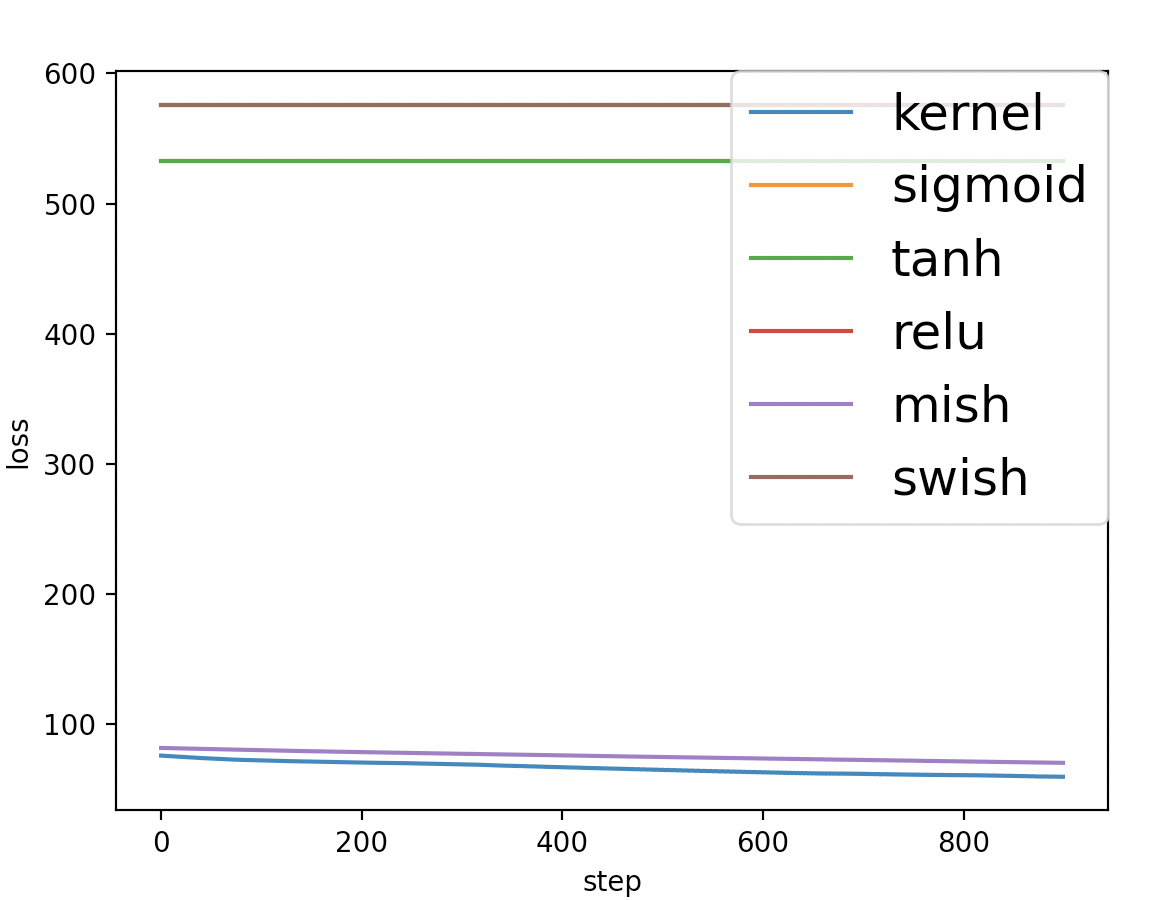
\includegraphics[clip, width=7cm]{asset/boston_0.00001_1000_3_005_sgd_non_xavier_uniform.png}
                    \caption{bostonの設定2の結果のValidationLoss}
                    \label{boston:loss_image2}
            \end{minipage}
        \end{tabular}
    \end{center}
\end{figure}


\subsubsection{bostonでの実験結果の考察}
bostonは本実験で唯一の回帰のデータセットである。

結果\ref{result:bostontable}を考察すると、ReLU等の関数よりも高い精度が出ることが判明した。





\subsection{breast\_cancerでの比較実験}
\label{ev:breastcancer}

\subsubsection{設定1及び設定2の結果}

breast\_cancerを用いた活性化関数の比較結果を表\ref{result:bostontable}に記す。


\begin{table}[htbp]
    \begin{center}
        \caption{breast\_cancerの設定1及び設定2のAccuracy}
        \label{result:breastcancer}
        \vspace{2mm} 
        \begin{tabular}{|c|c|c|}
            \hline
            活性化関数              & 設定1のAccuracy &  設定2のAccuracy \\
            \hline
            K-AF            & 43.0 & 90.3 \\
            \hline
            Sigmoid            & 47.3 & 78.3\\
            \hline
            Tanh            & 60.0 & 29.0\\
            \hline
            ReLU        & 43.0 & 29.0\\
            \hline
            Swish           & 55.3 & 42.6\\
            \hline
            Mish           & 47.3 & 42.6\\
            \hline
        \end{tabular}
    \end{center}
\end{table}




\subsubsection{設定1及び設定2のValidationLoss}
\label{breastcancer:loss}
ValidationLossのログデータを図\ref{breastcancer:loss_image1}と図\ref{breastcancer:loss_image2}に示す。


\begin{figure}[hbtp]
    \begin{center}
        \begin{tabular}{c}
            \begin{minipage}{0.5\hsize}
                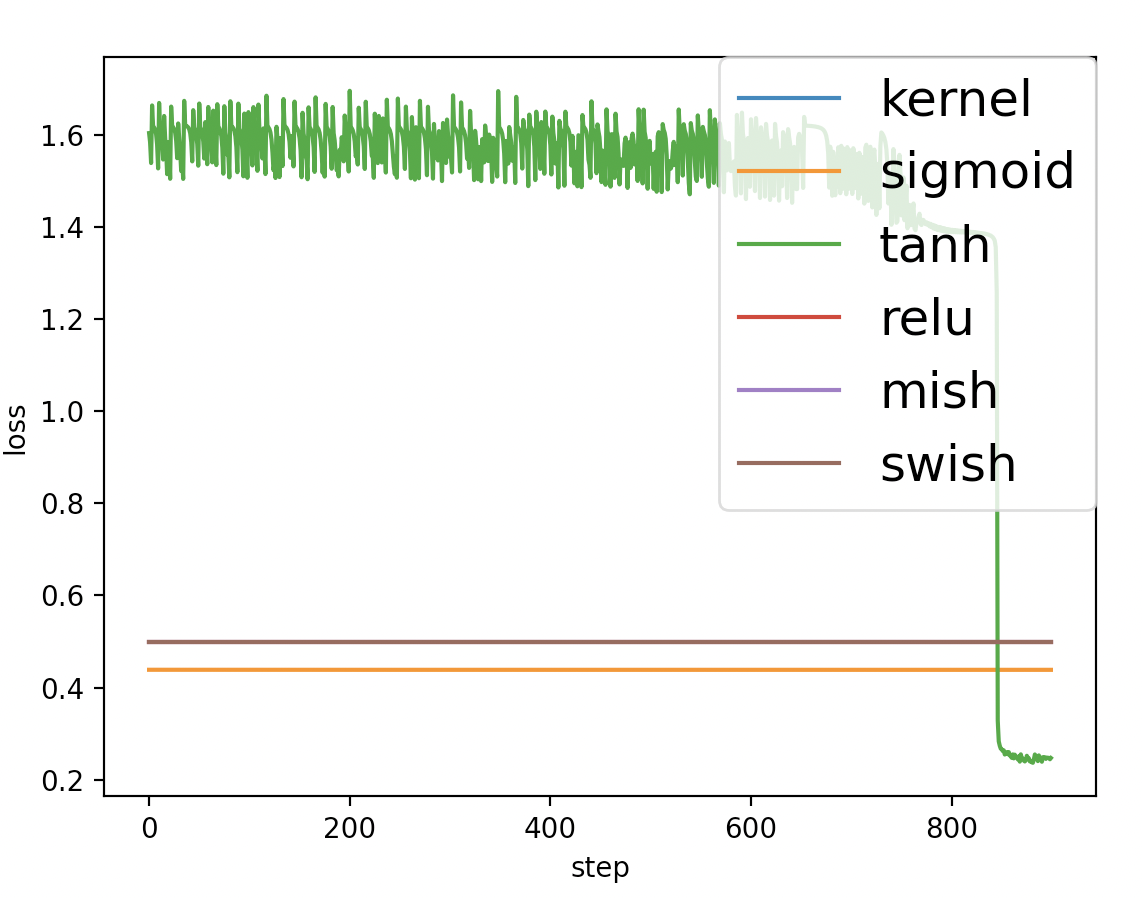
\includegraphics[clip, width=7cm]{asset/breastcancer_0.001_1000_3_005_sgd_non_kaiming_uniform}
                    \caption{breastcancerの設定1の結果のValidationLoss}
                    \label{breastcancer:loss_image1}
            \end{minipage}
            \hspace{10pt}
            \begin{minipage}{0.5\hsize}
                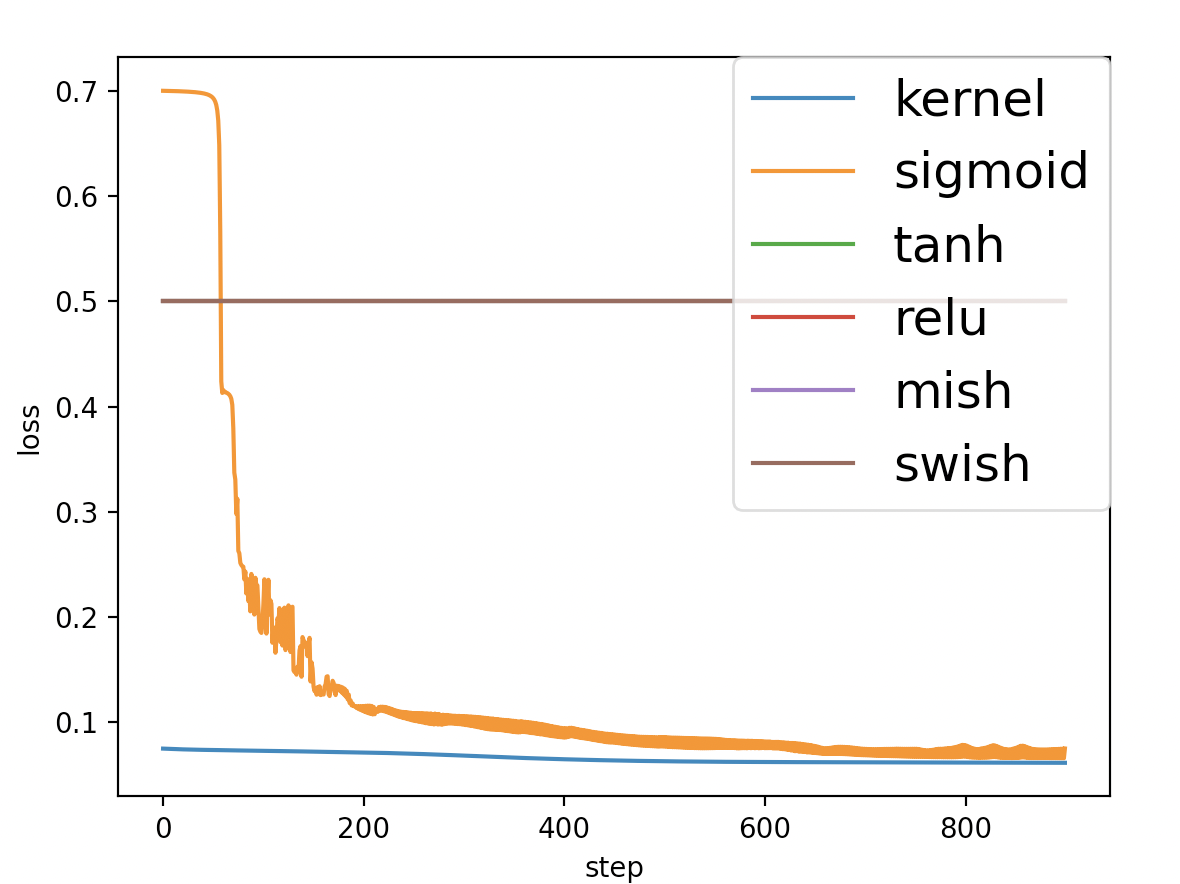
\includegraphics[clip, width=7cm]{asset/breastcancer_0.001_1000_3_05_sgd_non_kaiming_uniform}
                    \caption{breastcancerの設定2の結果のValidationLoss}
                    \label{breastcancer:loss_image2}
            \end{minipage}
        \end{tabular}
    \end{center}
\end{figure}


\subsubsection{breastcancerでの実験結果の考察}
結果\ref{result:breastcancer}を考察すると、勾配爆発が起きる条件に関わるものとして、カーネル密度関数を推定するためのデータセットの数が関与してることが明らかになった。
こちらも決定木の性能評価でよく使用されるデータセットであるため、ニューラルネットワークで評価をするのには向いていないことが精度が出づらいことの原因であると考えられる。
設定1での性能が極端に低い原因は計算用のデータセットの数が少ないことによる勾配爆発が原因であると考えられる。

\subsection{実験1全体のまとめ}
結果全体を考察すると、K-AFは本実験で使うようなデータセットの場合でも、いい条件で学習することができれば既存の活性化関数と同等もしくはより高い精度でどのデータセットも学習できることが判明した。
特に決定木の問題に対してもcalc\_numを多めに取ることができれば予想以上に高い精度を出すことが明らかになった。
複雑な問題に対しては、LearnigRateが大きい場合やcalc\_numが少ない場合はかなりの確率で勾配爆発を起こすことが判明した。


\section{実験2の結果 K-AFの関数形状の調査}
\label{evo2}
本節では、\ref{exp2}節で示した設定もとに実験を行い、\ref{af-class}の表を軸にどのような活性化関数になったか、損失を見ながら考察を行い結論を述べる。





\subsubsection{irisの活性化関数}
\label{evo2:iris_result}
実験の設定は表\ref{dataset_name}のLearningRateと表\ref{exp:iris}のLearningRate以外の設定を用いる。
推論した活性化関数の形は図\ref{infer_iris}のようになる。
\begin{figure}[hbtp]
    \begin{center}
        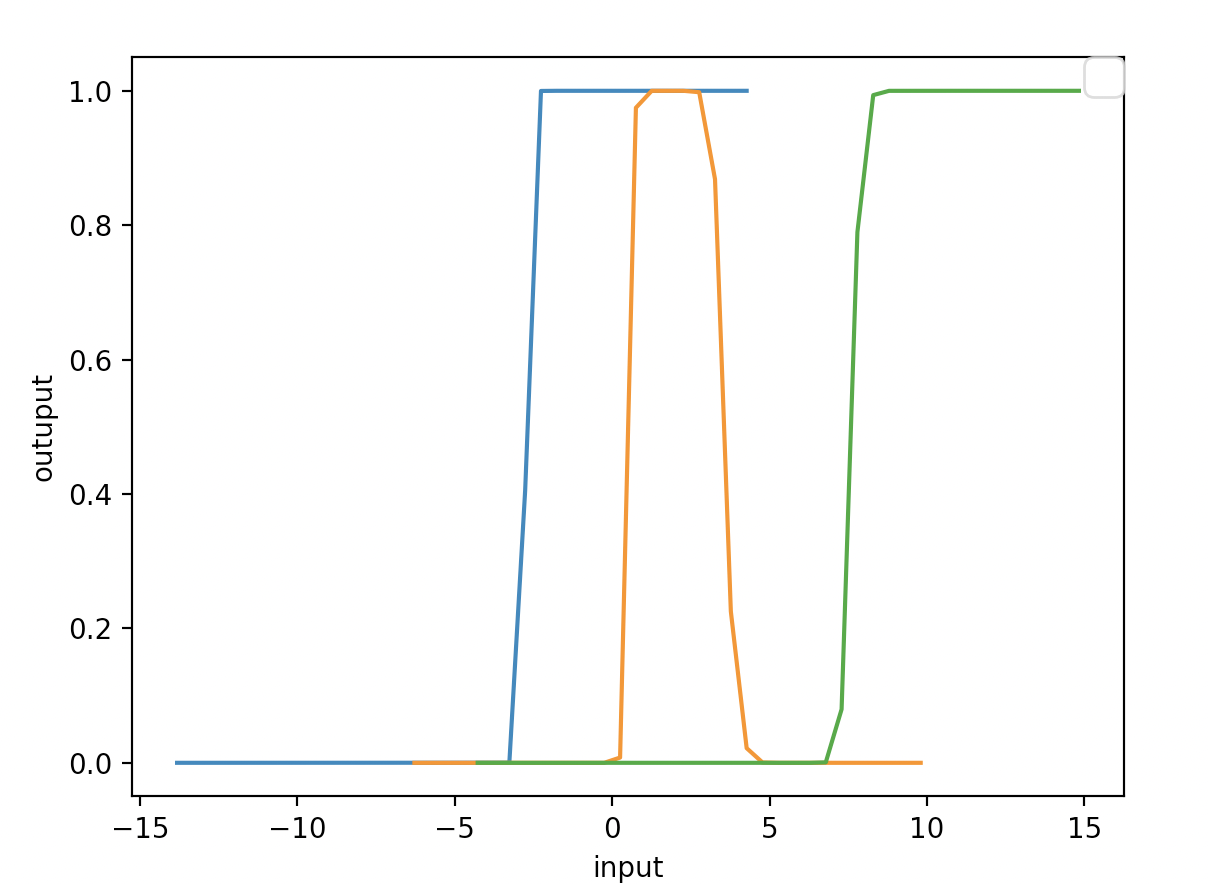
\includegraphics[width=10cm]{asset/iris-0.1.png}
            \caption{irisで推論した活性化関数の形}
            \label{infer_iris}
    \end{center}
\end{figure}

またこれを\ref{af-class}の表に当てはめると表\ref{anal_iris}のようになる。
\begin{table}[htbp]
    \begin{center}
        \caption{irisで推論した活性化関数の分析表}
        \label{anal_iris}
        \vspace{2mm} 
        \begin{tabular}{ |c|c| }
        \hline
        単調増加関数か & 上限値があるか   \\
        \hline
        × & ○   \\
        \hline
        \end{tabular}
    \end{center}
\end{table}



単純な分類問題であるが、\ref{infer_iris}を観察するにSigmoid等の活性化関数と違い単調増加もしくは単調減少しない活性化関数が導かれることが明らかになった。




\subsubsection{digitsの活性化関数}
\label{evo2:digits_result}
実験の設定は表\ref{dataset_name}のLearningRateと表\ref{exp:digits}のLearningRate以外の設定を用いる。
推論した活性化関数の形は図\ref{infer_digits}のようになる。
\begin{figure}[hbtp]
    \begin{center}
        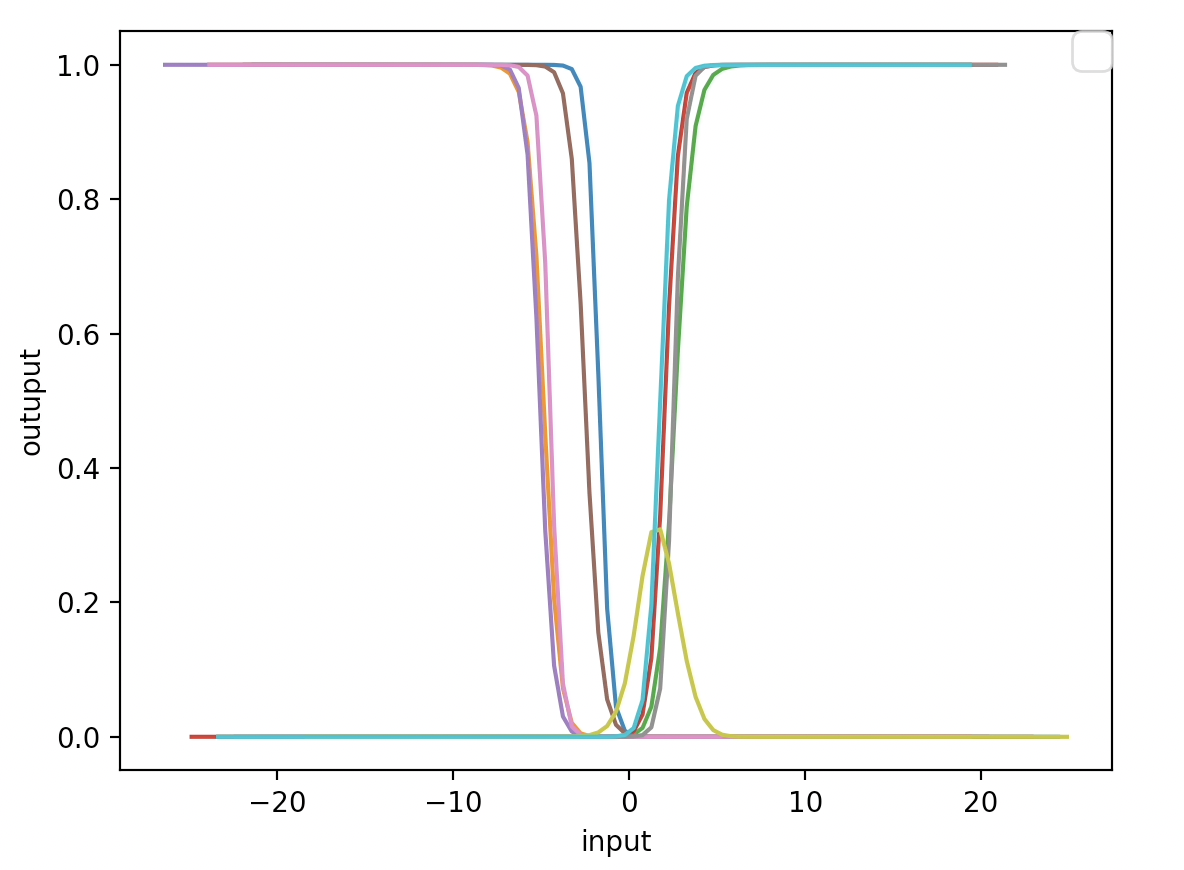
\includegraphics[width=10cm]{asset/digits-0.1.png}
            \caption{digitsで推論した活性化関数の形。出力層は10次元なので10個の関数が存在する。}
            \label{infer_digits}
    \end{center}
\end{figure}

またこれを\ref{af-class}の表に当てはめると表\ref{anal_digits}のようになる。
\begin{table}[htbp]
    \begin{center}
        \caption{digitsで推論した活性化関数の分析表}
        \label{anal_digits}
        \vspace{2mm} 
        \begin{tabular}{ |c|c| }
        \hline
        単調増加関数か  & 上限値があるか   \\
        \hline
        ▲ & ○   \\
        \hline
        \end{tabular}
    \end{center}
\end{table}

「単調増加関数か」が▲になる理由は単調増加とは対称的な単調減少の関数も推論した関数の中に存在するからである。
推論するデータセットがラベリング問題であるため上限値が$ 1 $であることから、このような形になったと考察できる。
例外的に一つ形が崩れているが、Sigmoidと関数の形がにているため、使用する関数としてもSigmoidのような形のもので十分な精度が出ることが予想できる。
実際に\ref{ev:wineでの実験と設定}ではSigmoidやTanhでも十分な性能を出している。


\subsubsection{wineの活性化関数}
\label{evo2:wine_result}
実験の設定は表\ref{dataset_name}のLearningRateと表\ref{exp:wine}のLearningRate以外の設定を用いる。
推論した活性化関数の形は図\ref{infer_wine}のようになる。
\begin{figure}[hbtp]
    \begin{center}
        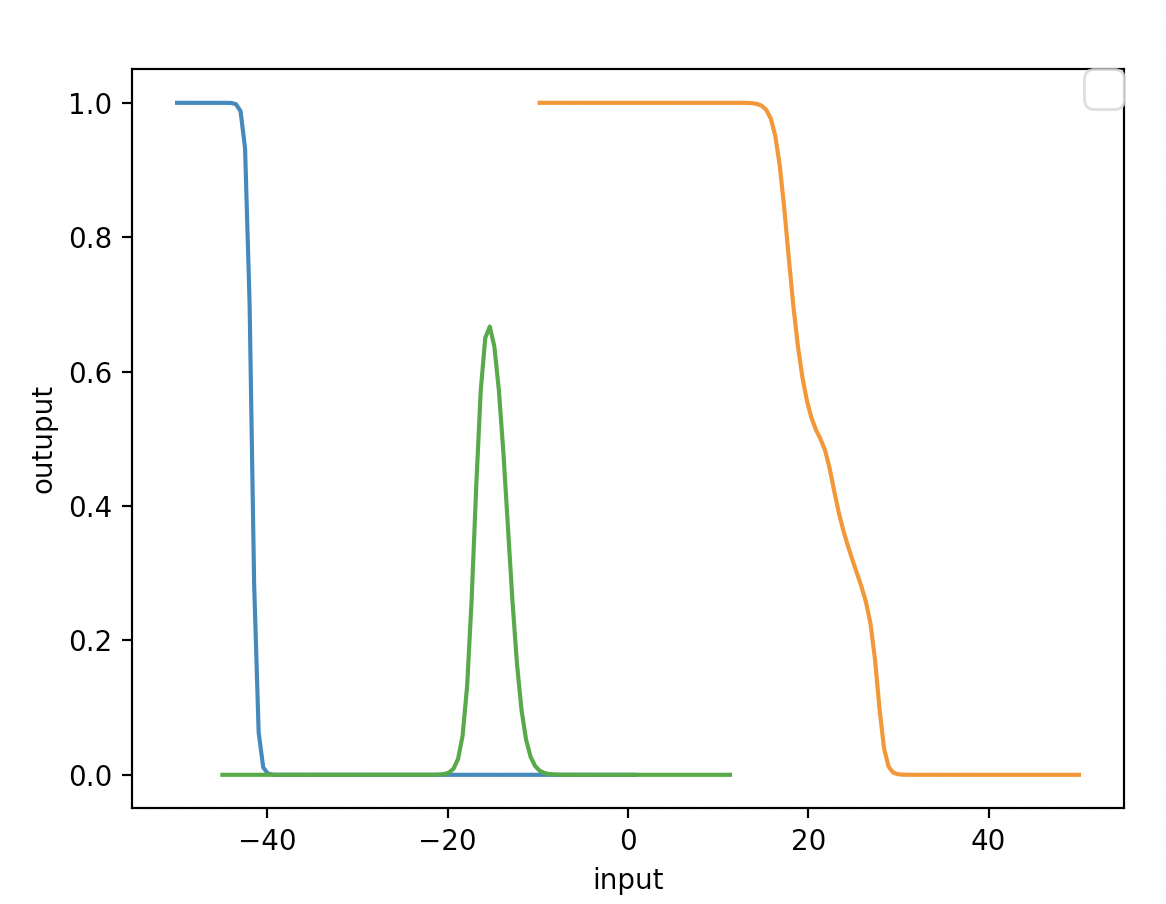
\includegraphics[width=10cm]{asset/wine-0.01.png}
            \caption{wineで推論した活性化関数の形。出力層が3次元なので3つの関数が存在する。}
            \label{infer_wine}
    \end{center}
\end{figure}

またこれを\ref{af-class}の表に当てはめると表\ref{anal_wine}のようになる。
\begin{table}[htbp]
    \begin{center}
        \caption{wineで推論した活性化関数の分析表。出力層が1次元の回帰問題なので、関数は一つだけである。}
        \label{anal_wine}
        \vspace{2mm} 
        \begin{tabular}{ |c|c| }
        \hline
        単調増加関数か  & 上限値があるか   \\
        \hline
        × & ○   \\
        \hline
        \end{tabular}
    \end{center}
\end{table}

K-AFでは高い性能を出すことができた。
分類問題であるためdigitsと同様に、上限が存在するが歪な形になっていることが確認できる。
これは決定木の性能評価のために使われるデータセットのため、ニューラルネットで表現できる関数空間との相性が悪いことが原因であると考えられる。






\subsubsection{bostonの活性化関数}
\label{evo2:boston_result}
実験の設定は表\ref{dataset_name}のLearningRateと表\ref{exp:boston}のLearningRate以外の設定を用いる。
推論した活性化関数の形は図\ref{infer_boston}のようになる。
\begin{figure}[hbtp]
    \begin{center}
        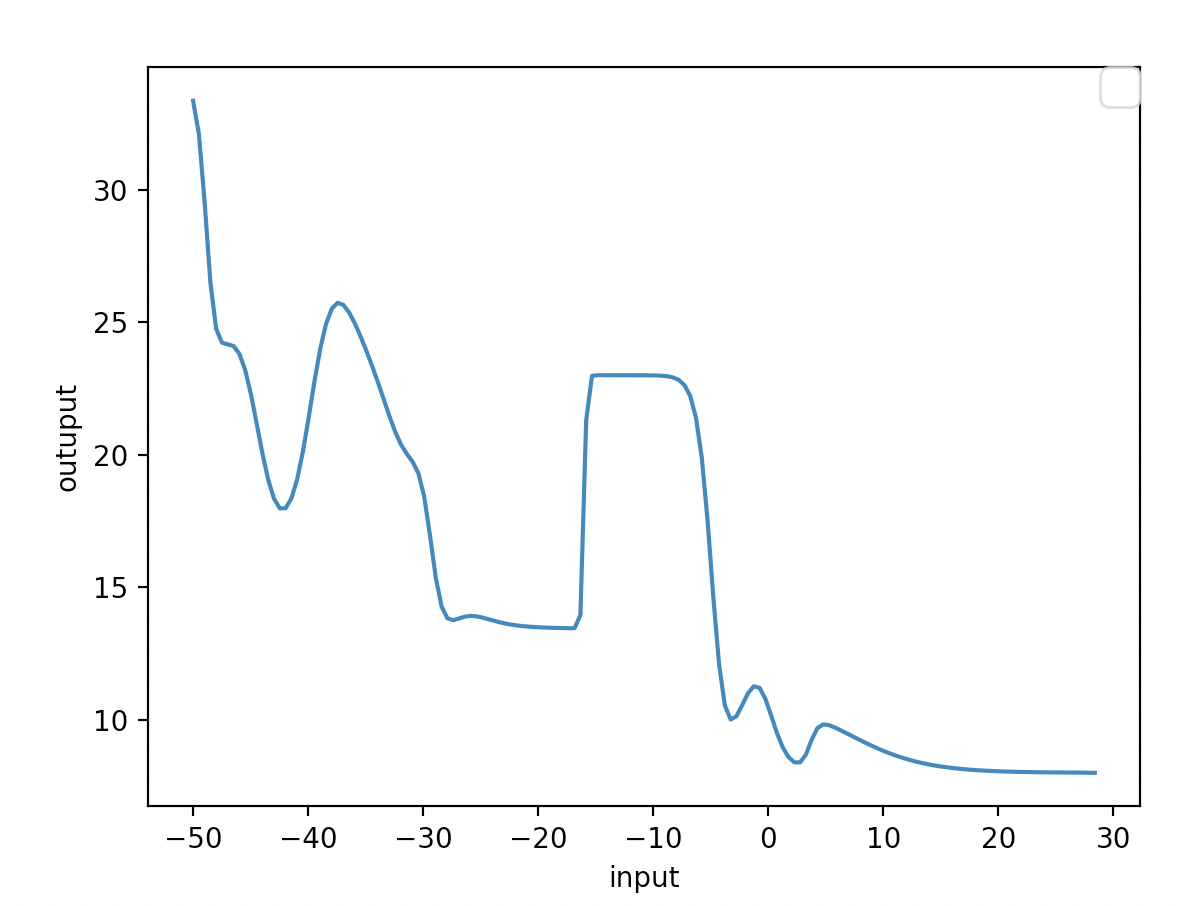
\includegraphics[width=10cm]{asset/boston-0.00001.png}
            \caption{bostonで推論した活性化関数の形}
            \label{infer_boston}
    \end{center}
\end{figure}

またこれを\ref{af-class}の表に当てはめると表\ref{anal_boston}のようになる。
\begin{table}[htbp]
    \begin{center}
        \caption{bostonで推論した活性化関数の分析表}
        \label{anal_boston}
        \vspace{2mm} 
        \begin{tabular}{ |c|c| }
        \hline
        単調増加関数か  & 上限値があるか   \\
        \hline
        × & ▲   \\
        \hline
        \end{tabular}
    \end{center}
\end{table}


bostonは回帰問題であるため、分類問題とは違い上限値が30になり、その中間の値も出力するようになった。
複雑な関数の形も推論できていることが確認できると同時に、このような問題に適した活性化関数がないことが原因でbostonでの実験\ref{ev:bostonでの比較実験}は非常に高い性能を出したのではないかと考察することもできる。
図\ref{infer_boston}のような形をした活性化関数は現状発表されてないので、既存の活性化関数では表現の幅が狭いことが確認できる良い例である。





\subsubsection{breastcancerの活性化関数}
実験の設定は表\ref{dataset_name}のLearningRateと表\ref{exp:breastcancer}のLearningRate以外の設定を用いる。
推論した活性化関数の形は図\ref{infer_breastcancer}のようになる。
\begin{figure}[hbtp]
    \begin{center}
        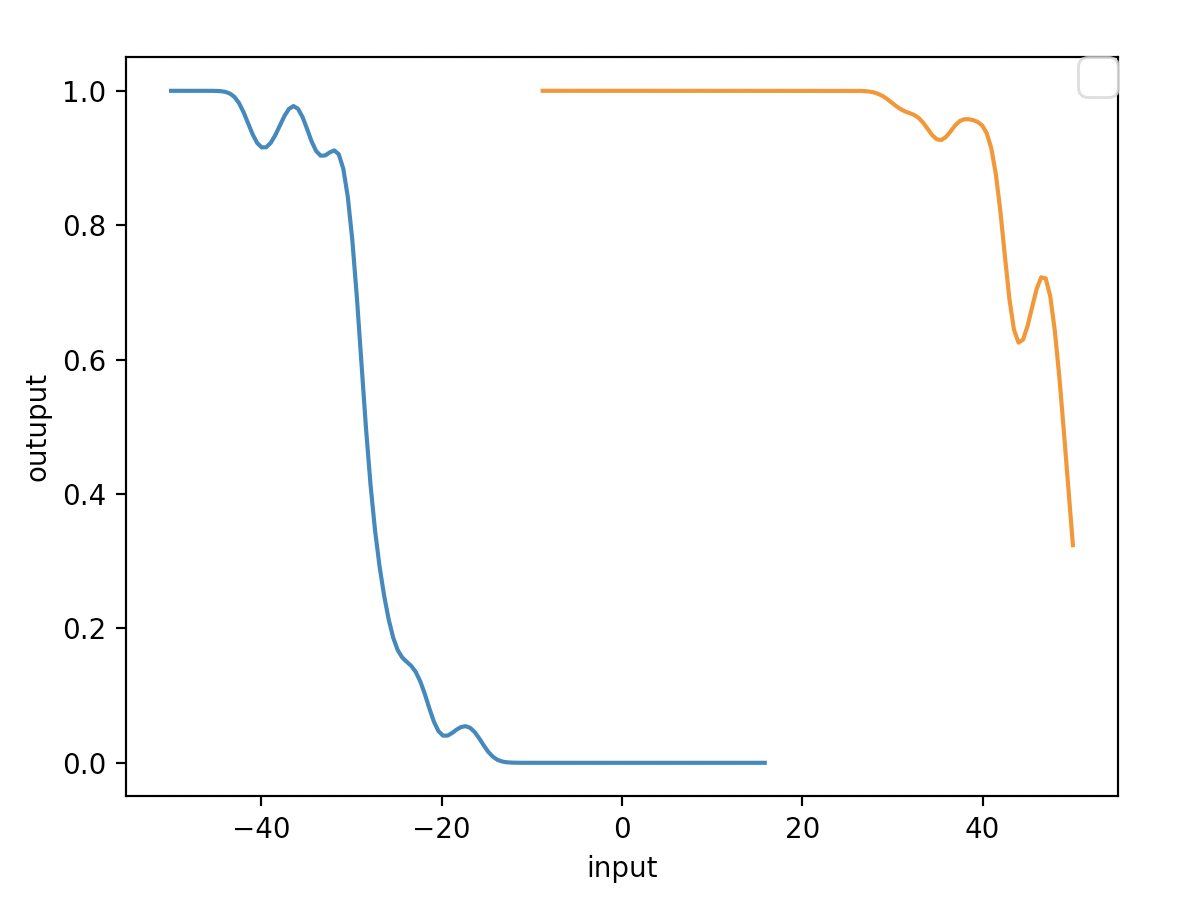
\includegraphics[width=10cm]{asset/breastcancer-0.01.png}
            \caption{breast\_cancerで推論した活性化関数の形}
            \label{infer_breastcancer}
    \end{center}
\end{figure}

またこれを\ref{af-class}の表に当てはめると表\ref{anal_breastcancer}のようになる。
\begin{table}[htbp]
    \begin{center}
        \caption{breastcancerで推論した活性化関数の分析表}
        \label{anal_breastcancer}
        \vspace{2mm} 
        \begin{tabular}{ |c|c| }
        \hline
        単調増加関数か  & 上限値があるか   \\
        \hline
        ▲ & ○   \\
        \hline
        \end{tabular}
    \end{center}
\end{table}


breast\_cancerは分類問題であるが決定木の評価に使われる関数である。
そのため、学習の不安定さ原因となり、LearnigRateが大きい場合や活性化関数に使うデータセットが少ない場合に勾配が爆発することが多かった。




\subsection{実験2全体のまとめ}
実験2\ref{evo2}により、K-AFが活性化関数を最適に推論してることが視覚的に理解できた。
また表\ref{af-class}を用いた分析により、決定木で使うようなデータセットの場合や回帰の場合などは既存の活性化関数では表現の幅が不足していることが判明した。

また、iris、digits、wine、bostonのK-AFの学習過程の動きをAppendix\ref{appendix:movie}で紹介している。









\section{実験3の結果 K-AFの性能が上がる条件探査}
\label{evo3}

本節では\ref{exp3}節で示した設定もとに実験を行い、一般的にどのような条件でK-AFがより良い性能を出すか、また、欠点が存在するかを\ref{evo3.1}項と\ref{evo3.2}項にて調査する。


\subsection{実験3.1 ニューラルネットワークの設定変更により精度向上の条件調査の結果}
\label{evo3.1}
\ref{exp3.1}項で示した比較実験の結果を記述する。


\subsubsection{bostonにおいて勾配爆発の確率の少ないニューラルネットワークの構成}
bostonのデータセットで最も性能が良かったニューラルネットワークの設定の上位5つを表\ref{bostonbest}に記述する。


\begin{table}[htbp]
    \begin{center}
        \caption{bostonを推論するときの最も勾配爆発確率が低いニューラルネットワークの設定の順位}
        \label{bostonbest}
        \vspace{2mm} 
        \begin{tabular}{ |c||c|c|c|c|c| }
        \hline
        順位 & Initializer & Optimizer &  Reguralizer & 勾配爆発回数 & 勾配爆発確率 \\
        \hline
        1 & Xavier & Adam & non & 275 & 27.5\% \\
        \hline
        2 & Xavier & Adam & l1 & 290 & 29.0\% \\
        \hline
        3 & Xavier & Adam & l2 & 294 & 29.4\% \\
        \hline
        4 & Xavier & SGD & l1 & 294 & 29.4\% \\
        \hline
        5 & Xavier & RMSprop & l1 & 298 & 29.8\% \\
        \hline
        \end{tabular}
    \end{center}
\end{table}


\subsubsection{性能評価まとめ}
表\ref{bostonbest}の順位を確認すると性能に直結しそうなものは初期値であり、上位の順位のものが全てXavierであることが明らかになった。
また、Appendixの表\ref{appendix:error}よりXavierはKaimingUniform によりもどの条件において勾配爆発の発生回数が半分程度だったことが判明した。
この議論において大切なことは、どのInitializer性能が向上したかということではなく、InitializerそのものがK-AFの性能に大きく影響しているということである。
Initializerの他には統計的な誤差の範囲内ではあるが、OptimizerとしてAdamを使用した場合にエラー頻度が低いことが明らかになった。

\subsection{実験3.2 クリッピングを用いた性能評価}
\label{evo3.2}
\ref{exp3.2}節で示した比較実験の結果を記述する。


\begin{table}[htbp]
    \begin{center}
        \caption{bostonを用いたK-AFにクリッピングを用いた際の勾配爆発の回数と確率}
        \label{clipping_boston}
        \vspace{2mm} 
        \begin{tabular}{ |c|c|c| }
        \hline
        構成 & 勾配爆発の回数 & 勾配爆発の確率\\
        \hline
        クリッピングなし  & 648 & 64.8\% \\
        \hline
        クリッピングあり  & 590 & 59.0\% \\
        \hline
        \end{tabular}
    \end{center}
\end{table}



\subsubsection{クリッピングの性能まとめ}
\ref{clipping_boston}節の結果により、クリッピングがK-AFの勾配爆発の確率を減らすことには直接影響しないことが明らかになった。



\subsection{実験3まとめ}
実験3.1により、K-AFの性能を引き出す最大の要素はInitializerに関わっていることが明らかになった。
これは初期値の段階で勾配爆発に陥ってる可能性が高いことが原因であると考えられる。


%%% Local Variables:
%%% mode: japanese-latex
%%% TeX-master: "./thesis"
%%% End:
